\chapter{Introduction}
\label{intro}

This chapter provides a background into the motivation behind the
development of the \agentj~framework.  AgentJ is essentially a 
Java Virtual Machine (JVM) for the NS2 simulation environment \cite{ns2}. It allows
multi-thread Java networked applications without modification to be 
orchestrated and run within multiple network configurations in the NS-2
discrete time simulator. This enables Java networked applications to
be stress-tested under certain networked conditions before deployment
and new research ideas to be proved and demonstrated through 
performance or functional analysis and visualisation.  AgentJ
contains a number of UDP, multiucast and TCP examples to
demonstrate its usage and it also contains more complex scenarios
that contain multiple sockets and threads.   

\index{JVM}\index{Protolib}\index{P2PS}\index{P2P}
\index{NS-2}

AgentJ contains a bytecode rewriting subsystem that swaps user 
code on-the-fly to use its own implementations of network, threading and
timing functions for use within Ns-2. AgentJ therefore contains
a complete native implementation for the \emph{java.net} package
via a toolkit called Protolib for integration with NS-2 and also overrides 
several key objects within the core JVM including 
\emph{java.lang.Thread} and even \emph{java.lang.Object}. Below are a list of the key features of the system.  AgentJ:

\index{Bytecode Rewriting}

\begin{itemize}
\item Manages sockets, network addresses, threads, thread synchronisation (wait and notify), timers (Thread.sleep+ others)
\item Includes a ns-2 DNS server and a re-implementation of the sockets from java.net.*
\item Re-implements java.lang.Thread - for overriding t java threads. Since Ns-2 is not multi-threaded, AgentJ needs to monitor all threads created by the application and internally control their synchronicity.  
\item Incorporates a re-implementation of java.lang.Object for Java monitors.
\item Consists of a combination of bytecode rewriting and aspect-oriented techniques to dynamically swap the run-time environment for Java networked applications, by:
\begin{itemize}
\item performing a find/replace on the bytecode on various packages, e.g. java.net, some key classes java.lang.Object and some classes in java.io.
\item using Javassist to replace some method-level invocations for wait() and notify(), for overloading start() and run() for thread synchronisation and for timing operations e.g. java.lang.Thread.sleep().
\end{itemize}
\item Includes a number of real-world including demos of P2PS Simulations, a complex multi-threaded middleware, without modification of the source code.
\end{itemize}

\section{Motivation for \agentj}


\agentj~has been developed primarily by Ian Taylor\footnote{Ian.J.Taylor@cs.cardiff.ac.uk}, who has  been working with
the PROTEAN Research Group in NRL for the past six years 
(with PIs Brian Adamson and Joe Macker, and earlier also involving 
Rick Jones).  Other key contributors 
to the project include Ian Downard\footnote{iandownard@ieee.org}, 
Ian Wang\footnote{ianwangcardiff@googlemail.com} and Andrew 
Harrison\footnote{Andrew.Harrison@cs.cardiff.ac.uk}. The PROTEAN Research Group 
has used AgentJ in a variety of projects working dynamic 
networking protocol and middleware issues  including
SRSS ( Scalable Robust Self-organizing Sensor), MODAN 
(Multi-agent systems Operating within Dynamic Ad 
hoc Networks), and currently SONOMA (Service Oriented 
Networking Operating in Mobile Ad hoc) Networks. 

One main theme for all of these projects has been to investigate 
and model, using network simulation tools, lightweight network 
application discovery mechanisms suitable for application in 
mobile sensor systems,  leveraging self-organizing computer 
communication networks where possible, based on Mobile 
Ad-hoc Networking (MANET) routing protocols which operate 
using wireless communication links and 
have no centralized administration or control.  The PROTEAN group 
have been considering a complexity of middleware approaches, 
from simple network services e.g. network name/address 
resolution, IP multicast, ANYCAST,  to potentially heavy-weight, 
highly stateful, complex agent-based architectures. However, the focus 
is on relatively lightweight (minimally complex) middleware discovery 
mechanisms and services which can facilitate �publish and subscribe� 
relationships among a set of sensor application peers participating 
in an MANET network.  To this end, we developed AgentJ in
order to provide a framework for investigating the possible 
Java middleware solutions. This work led to some initial
tests investigating common peer-to-peer (P2P) techniques for dynamically 
discovering and connecting the mobile sensor nodes.    

\index{PROTEAN Group}
\index{MANET}
\index{P2P}

P2P applications typically create virtual network overlays for connecting 
users from highly transient devices and computers behind NAT, firewalls, 
etc, often referred to as peers at the \emph{edges of the Internet}  
\cite{Shirky2000}.  P2P applications and middleware e.g. Jxta \cite{jxta},
typically use a combination of discovery techniques in order to connect 
peers in more decentralised nature than conventional Web-based applications.
In the first instance we looked at \emph{unstructred P2P approaches} and 
the P2PS middleware \cite{p2ps} was selected over potentially more 
complex systems such as Jxta, because we had strong in-house 
support for the software.  The unstructured P2P approach is interesting 
because it attempts to address similar unreliable connectivity issues to 
mobile sensor environments. However, in this regard sensor nets
can be more extreme, where nodes not only 
disappear/reappear frequently, but data rates are continuously changing 
as the sensors move away from the wireless hubs and other factors, such as 
battery strength, can affect the type of role the sensor can 
play within the network. 

\index{NAT}
\index{P2PS}
\index{P2PS}




\begin{figure}[htbp]
\begin{center}
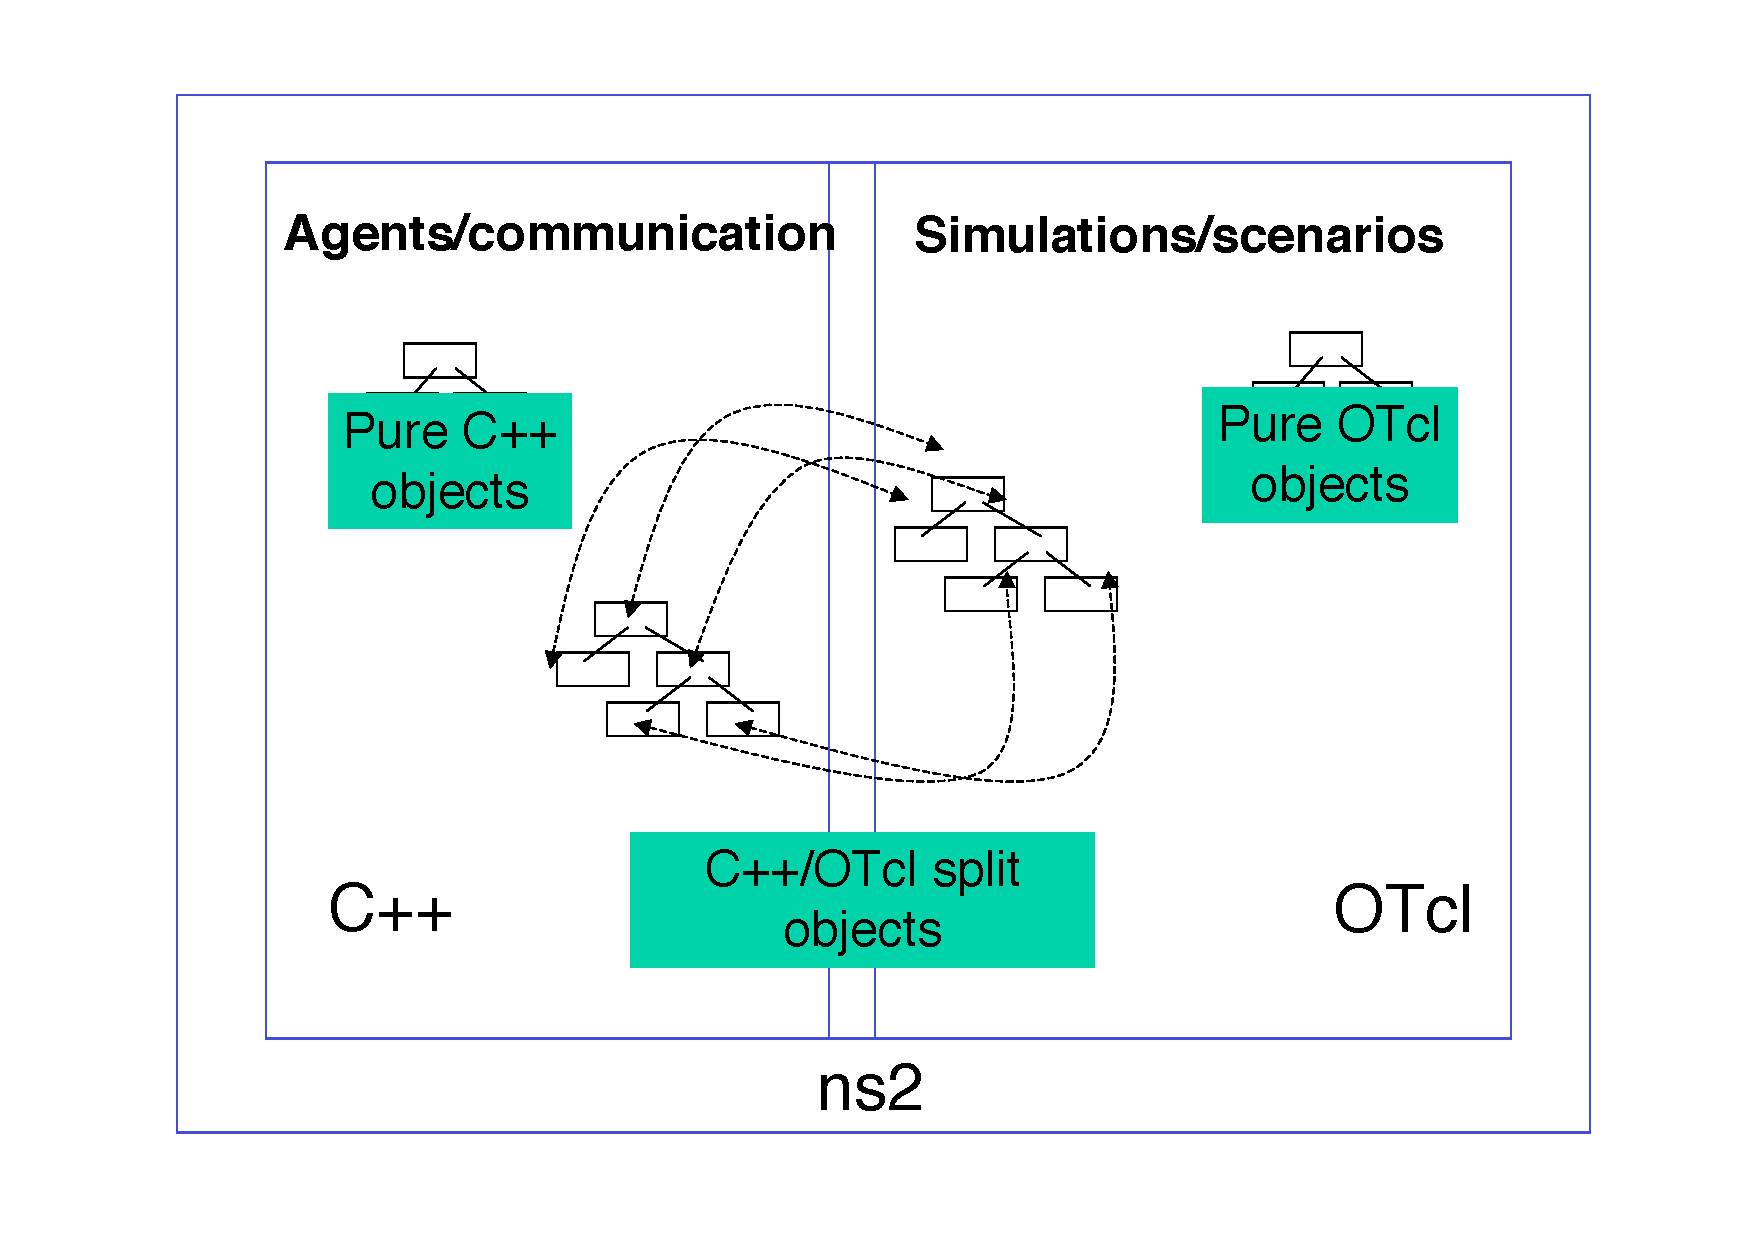
\includegraphics[scale=0.40]{images/nsoverview}
\caption{Ns-2 Component Overview}
\label{intro:fig:nsoverview}
\end{center}
\end{figure}

\section{NS-2, Protolib and AgentJ}
\label{sec:nsprotolib}

\index{Ns-2}

NS-2 \cite{ns2} is a discrete event simulator that supports the link layer upwards 
on the OSI stack i.e. the network, transport, session, presentation 
and application layer, respectively. It can support both wired and wireless 
simulations and works on most platforms and therefore satisfies 
the main focus of the project, that is, to test out various 
P2P discovery and communication mechanisms within various 
network extremities. NS-2 builds on years of experience and contains a 
number of existing transport protocols, written in a combination of
C++ and Tcl. The simulation network configuration and orchestration 
is written in Tcl, the Ns-2 engine is written as a mixture of Tcl (oTcl) and C++
and the underlying protocols are written mostly in C++ with some 
configuration in Tcl.   A rough schematic is provided in Figure 
\ref{intro:fig:nsoverview} illustrating these relationships. 

The Ns-2 environment was designed for simulating traffic, rather than deal
with the content of the traffic. Therefore, in the Protolib toolkit  \cite{protolib}, 
we have extended this vision to implement fairly complete versions of the UDP, 
Multicast and TCP protocols that permit the sending of payload traffic, which 
is necessary for message-based systems like P2P and publish/subscribe.  
For TCP in particular, we have implemented the full range of 
TCP event handshaking to model real-world TCP behaviour and we have 
included full support for TCP servers that can handle multiple connections.  
AgentJ implements its native Java networking binding directly to the
Protolib toolkit for interfacing with Ns-2. This is illustrated in Figure
\ref{intro:fig:layers}.

\begin{figure}
\centering
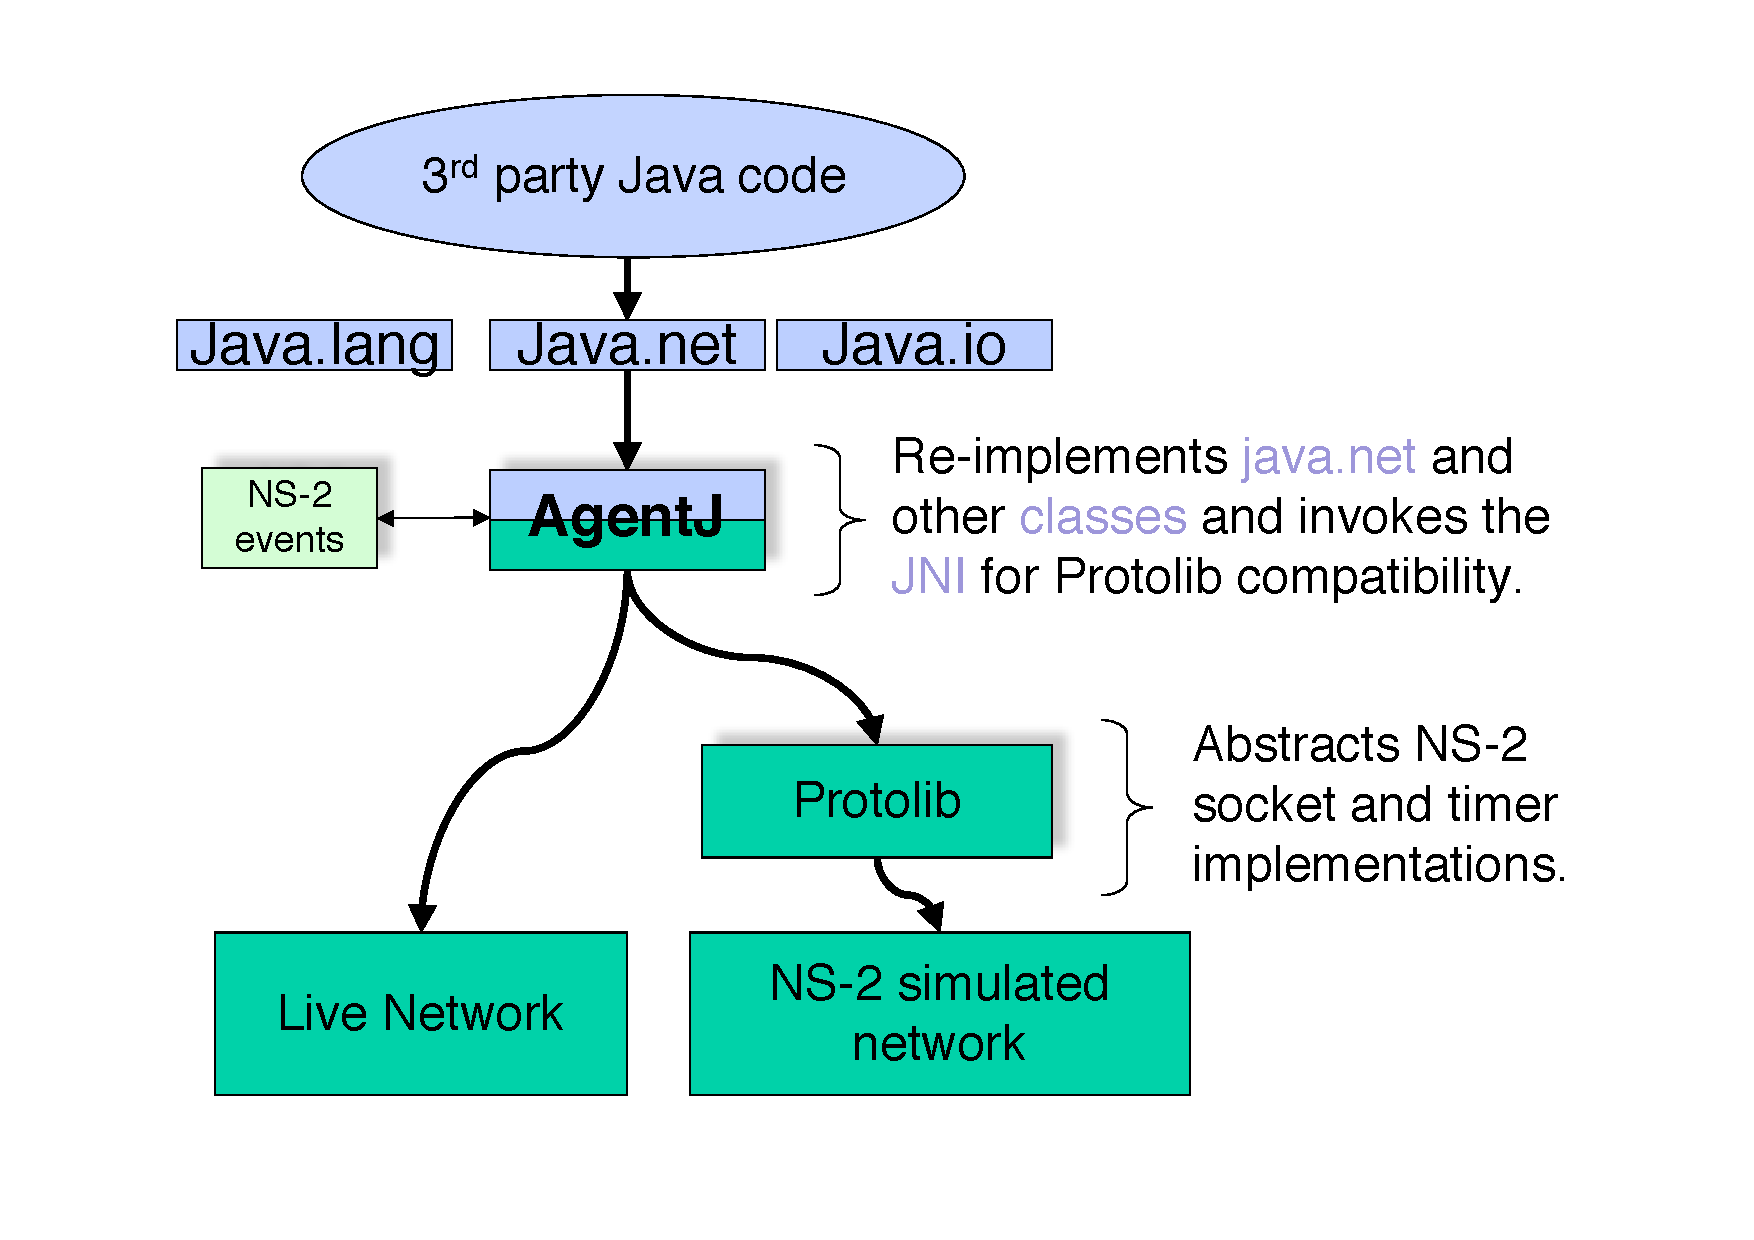
\includegraphics[scale=0.49]{images/agentjoverview}
\caption{An overview of the \agentj~software stack} 
\label{intro:fig:layers}
\end{figure}

\index{Protolib}

Protolib implements a switchable communications layer for several 
communication protocols (e.g. TCP, UDP, Multicast etc) in that
the same programming interface can be used to communicate 
within NS-2, OPNET and a networked environment. To bind to a 
particular environment, typically the application just needs to be 
recompiled.  \agentj~re-implements the Java networking, io and
threading layers of Java to work with the Protolib toolkit, switched in 
its NS-2 mode. For networked applications, AgentJ can just switch
itself off and Java will default to its conventional native implementations  
as illustrated.  Since Protolib contains a consistent socket and timer
interface to each of its supported environments it would mean
that AgentJ could potentially work in OPNET through a 
recompilation of the underlying shared libraries.  Future work may investigate
this possibility. 

The main thrust of AgentJ lies in the switching between the Java native 
implementations of its network core and the implementation
for NS-2 in Protolib. This is unfortunately non-trivial because there
is no such interface in java.net that allows socket implementations
to be swapped whilst using non-IP addresses.  The current 
\emph{SocketImpl} and \emph{SocketImpl} mechanism is 
tied closely into the IP address format, which is not possible to extend
to include Ns-2 address scheme (that uses simple integers).  
Therefore, AgentJ uses bytecode rewriting to provide similar
but alternative implementations to create hooks into java.net for
access to the different addressing scheme and for implementing
a new native implementation for this package.

\index{Bytecode Rewriting}
\index{JNI}
\index{J-Sim}
\index{PeerSim}

The result is that Java implementations running in AgentJ are
bytecode re-written at run-time in order to invoke
the AgentJ native implementation.  This means that no prior
configuration of alteration of the original source code needs
to be undertaken to run these codes in AgentJ.  This is
a different approach that has been undertaken by other projects
(e.g. J-Sim \cite{jsim} or PeerSim \cite{peersim}) which 
involve rewriting a version of an application for simulation.
 



